\chapter{Introduction}

\section{Background and Recent Research}
Optical character recognition is the mechanical or electronics conversion of images of types, handwritten or printed text into machine-encoded text, whether from a scanned document, a photo of a document, a scene-photo or from subtitle text superimposed on an image. It is widely used as a form of information entry from printed paper data records from passport documents, invoices, bank statements, computerized receipts, business cards, mail, printouts of static-data, or any suitable documentation. It is a common method of digitizing printed texts so that they can be electronically edited, searched, stored more compactly, displayed online, and used in machine processes such as cognitive computing, machine translation, (extracted) text-to-speech, key data and text mining. OCR is a field of research in pattern recognition, artificial intelligence and computer vision.

In the early days, the OCR systems needed to be trained with images of each characters, and worked on one font at a times. But now advance systems capable of producing high degree of recognition accuracy for most fonts are now common, and with support for a variety of digital image file format inputs. In 2006, Geoffry Hinton et al. published a paper [1] showing how to train a deep neural network capable of recognizing handwritten digits with state-of-the-art precision (>98\%). They branded this techniques “Deep learning”. Since then many advanced algorithms have been implemented not only to recognize but also to identify and segment texts in images. 

\subsection{Problem Statement}
The major problem with the OCR systems today is that they are trained with only a small number of fonts and thus cannot predict accurately the characters written in various other fonts. The problem is even more serious in case of handwritten digits which are even harder to recognize as each individual has a completely different style of writing and thus a unique character representation in their writing. This makes the job of OCR systems much more difficult. 

In the present world, many of the human tasks are being automated and equipped with machine intelligence. This means machines need to see and understand the outside world as we humans do. That is why, they need to identify objects, texts, from images and interpret them just like we do. For this a robust and accurate system to identify and classify texts is needed. So in this project an OCR system capable of recognizing handwritten and printed digits has been developed. 

There are OCR systems already in the market but they are very specific in their inputs. They are specific to one or two fonts, and require perfect lighting conditions and orientation of the characters in the image.

This system is different from the present systems because it has been trained on various datasets consisting of letters in varieties of fonts, colors and sizes. It has been developed with the convolutional neural networks which are great for efficient learning of features from images and classifying them. Also a number of preprocessing is performed in the image before it is send to the prediction model. This considerably reduces the errors for the prediction model and thus improves its accuracy.

\subsection{Objectives}
\begin{itemize}
\item Develop an OCR system to automate problems like digitizing forms, documents, data entry, etc.
\item Develop an OCR system to recognize handwritten as well as printed digits
\end{itemize}

\section{Motivation}
The major problem with the OCR systems today is that they are trained with only a small number of fonts and thus cannot predict accurately the characters written in various other fonts. The problem is even more serious in case of handwritten digits which are even harder to recognize as each individual has a completely different style of writing and thus a unique character representation in their writing. This makes the job of OCR systems much more difficult. 
In the present world, many of the human tasks are being automated and equipped with machine intelligence. This means machines need to see and understand the outside world as we humans do. That is why, they need to identify objects, texts, from images and interpret them just like we do. For this a robust and accurate system to identify and classify texts is needed. So in this project an OCR system capable of recognizing handwritten and printed digits has been developed. 
There are OCR systems already in the market but they are very specific in their inputs. They are specific to one or two fonts, and require perfect lighting conditions and orientation of the characters in the image.
This system is different from the present systems because it has been trained on various datasets consisting of letters in varieties of fonts, colors and sizes. It has been developed with the convolutional neural networks which are great for efficient learning of features from images and classifying them. Also a number of preprocessing is performed in the image before it is send to the prediction model. This considerably reduces the errors for the prediction model and thus improves its accuracy.

\section{Literature Review}
There are many methods that are applied in text extraction and recognition. Maximally Stable Extremal Regions along with canny edge detection has been used as a method of text detection in images [2]. The approach used by us is partly based on [3] which concerns only with the recognition of Devanagari characters using a CNN architecture. In addition to that an image pre-processor is used to enhance further the accuracy of the CNN architecture.

We have tried to combine the concepts of the two in our system. 
    \subsection{Maximally Stable Extremal Regions and Canny Edge Detector}
    
MSER has been identified as one of the best region detectors due to its robustness against view point, scale, and lighting changes. But it is sensitive to image blur. To cope with blurred images, the complimentary property of Canny edges is combined with MSER to enhance its performance. The outline of extremal regions can be enhanced by applying the precisely located but not necessarily connected Canny edges. i.e. the MSER pixels outside the boundary formed by the Canny edges are removed.

    \subsection{Convolutional Neural Networks}
Deep Neural Networks do not require any feature to be explicitly defined, instead they work on the raw pixel data generating the best features and using it to classify the inputs into different classes. Deep Neural Networks consist of multiple nonlinear hidden layers so the number of connections and trainable parameters are very large. Besides being very hard to train, such networks require a very large set of examples to prevent overfitting. One class of DNN with comparatively smaller set of parameters and easier to train is Convolutional Neural Networks. The ability of CNN to correctly model the input dataset can be varied by changing the number of hidden layers and the trainable parameters in each layer and they also make correct assumption on the nature of images. 

Like a standard feed forward network, they can model complex non-linear relationship between input and output. But CNN have very few trainable parameters than a fully connected feed-forward network of same depth. CNNs introduce the concept of local receptive field, weight replication and temporal subsampling which provide some degree of shift and distortion invariance. CNNs for image processing generally are formed of many convolution and sub-sampling layers between input and output layer.


\section{Theoretical Background}
    \subsection{Convolutional Neural Networks:}
Convolutional Neural Network (CNN or ConvNet) is a biologically inspired trainable machine learning architecture that can learn from experiences like standard multilayer neural networks. ConvNets consist of multiple layers of overlapped tiling collections of smaller neurons to achieve better representation of the original image. ConvNets are widely used for image and video recognition. There are three main types of layers used to build a ConvNet architecture.

        \begin{enumerate}
        \item Convolution Layer
        
The convolution layer is the core building block of a convolutional neural network. It convolves the input image with a set of learnable filters or weights, each producing one feature map in the output image.

        \item Pooling Layer
        
The pooling layer is used to progressively reduce the spatial size of the representation to reduce the amount of parameters and computation in the network. The pooling layer takes small rectangular blocks from the convolution layer and subsamples it to produce a single output from the block. There are several ways to do this pooling, such as taking the average or the maximum, or a learned linear combination of the neurons in the block.

        \item Fully-Connected Layer
        
The fully connected layer is used for the high-level reasoning in the neural network. It takes all neurons in the previous layer and connects it to every single neuron it has. Their activations can be computed with a matrix multiplication followed by a bias offset as a standard neural networks.

\end{enumerate}

\begin{figure}[htb]
\centering
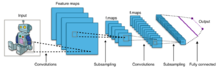
\includegraphics{220px-Typical_cnn}
\caption{Typical CNN architecture}
\end{figure}

    \subsection{ Maximally Stable Extremal Regions}
Maximally Stable Extremal Regions (MSER) is a feature detector. The MSER algorithm extracts from an image a number of co-variant regions, called MSERs. An MSER is a stable connected component of some level sets of the image. Optionally, elliptical frames are attached to the MSERs by fitting ellipses to the regions.
    \subsection{ Canny Edge Detection}
The Canny Edge detector is an edge detection operator that uses a multi-stage algorithm to detect a wide range of edges in images. It is a technique to extract useful structural information from different vision objects and dramatically reduce the amount of data to be processed. The process of Canny edge detection algorithm are:
        \begin{enumerate}
        \item Apply Gaussian filter to smooth the image in order to remove the noise
        \item Find the intensity gradients of the image
        \item Apply non-maximum suppression to get rid of spurious response to edge detection
        \item Apply double threshold to determine potential edges
        \item Track edges by hysteresis: finalize the detection of edges by suppressing all the other edges that are weak and not connected to strong edges.
        \end{enumerate}
